\chapter{绘制杯立体图}\label{chap:bei}

{\bfseries 学习目标}
\begin{itemize}
\item 学习利用Line命令和circle命令绘制图形
\item 学习利用offset命令和trim命令绘制图形
\item 学习利用region命令、revolve命令和extrude命令进行物体的三维建模
\item 掌握视图的基本概念
\item 掌握AutoCAD坐标的运用方法
\item 掌握物体三维建模的基本要领
\end{itemize}

{\bfseries 任务要求}
\begin{itemize}
\item 根据图\ref{fig:tiaoyafabei}所示的杯零件图,用旋转法建立调压阀杯零件的三维模型
\item 根据图\ref{fig:tiaoyafabei}所示的杯零件图,用拉伸法建立调压阀杯零件的三维模型
\end{itemize}

\noindent
\begin{figure}[htbp]
\centering
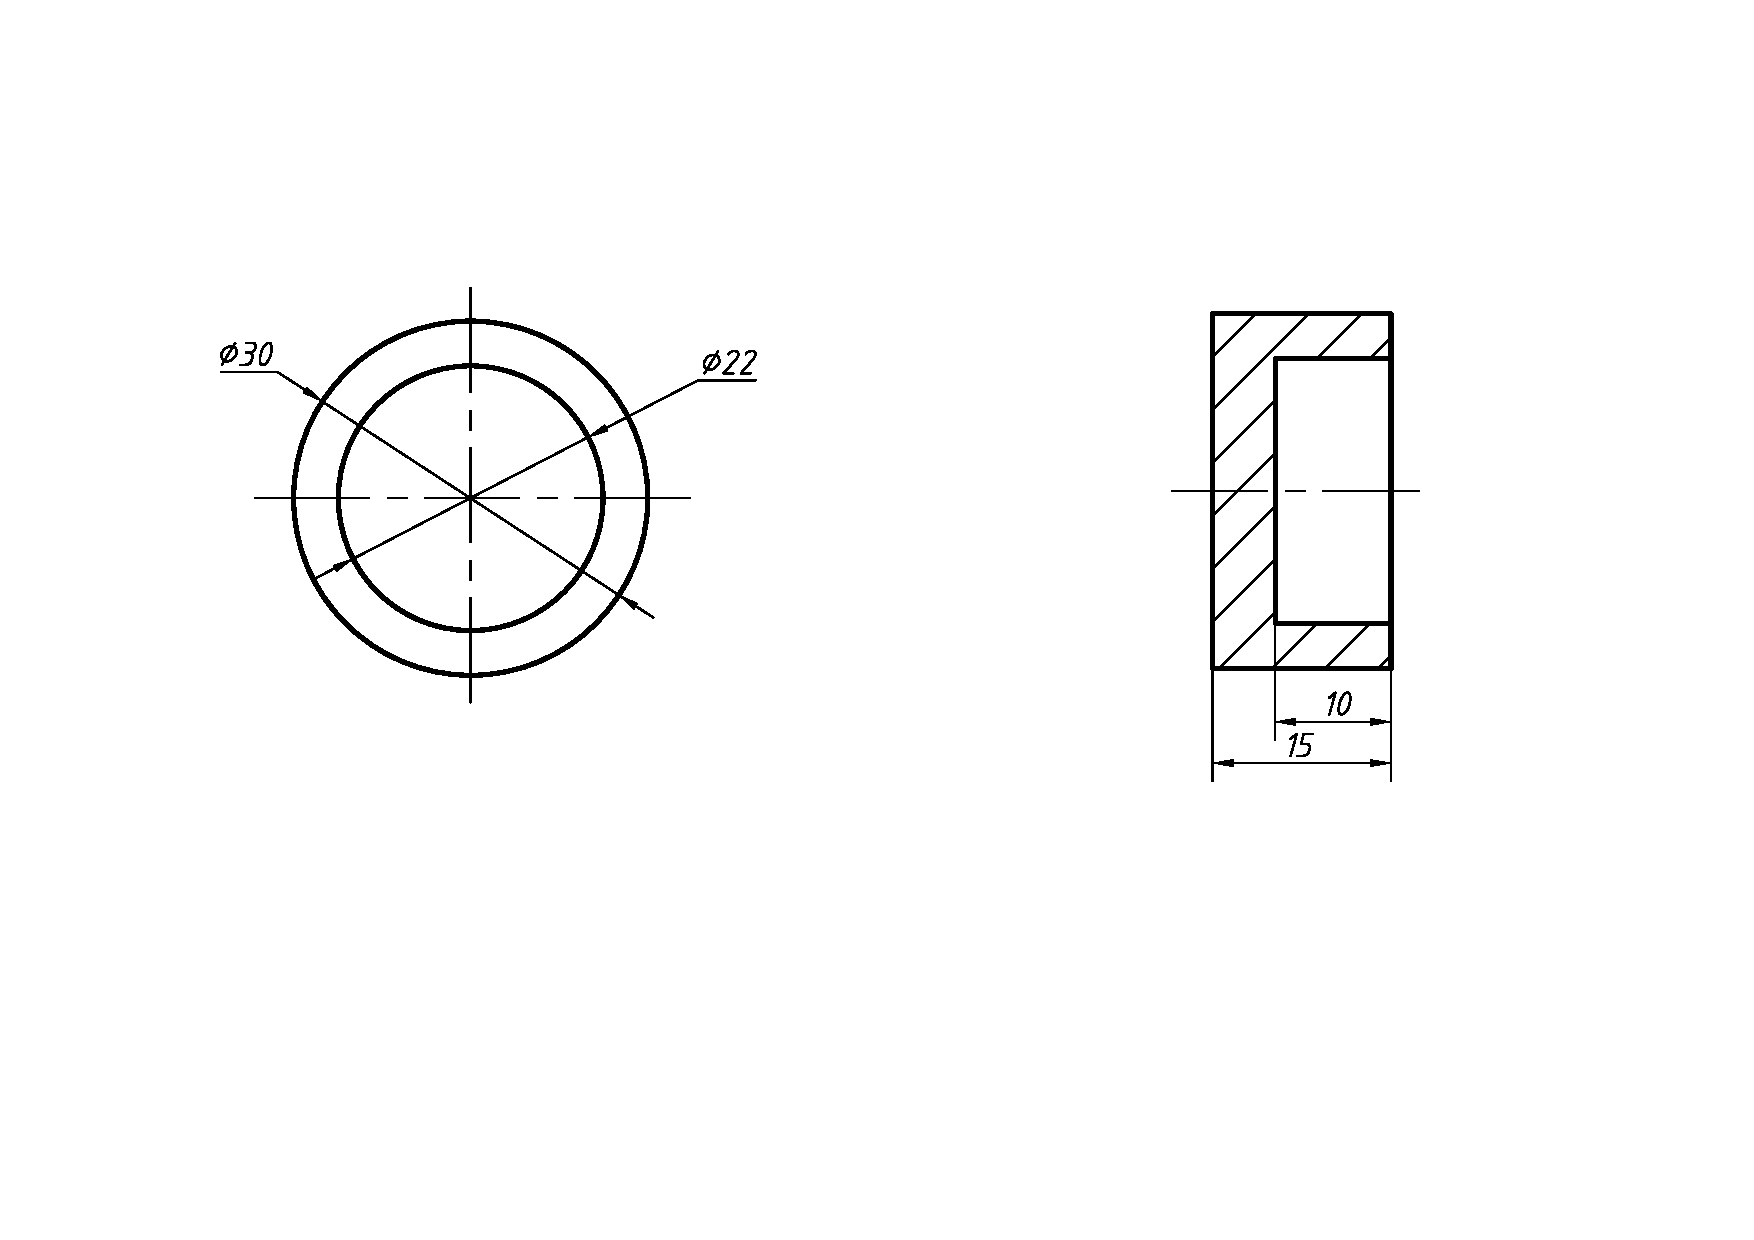
\includegraphics[scale=0.6]{tiaoyafabei.pdf}
\caption{杯零件图}\label{fig:tiaoyafabei}
\end{figure}
\endinput